\documentclass{beamer}
\usepackage{amsmath}
\usepackage[english]{babel} %set language; note: after changing this, you need to delete all auxiliary files to recompile
\usepackage[utf8]{inputenc} %define file encoding; latin1 is the other often used option
\usepackage{csquotes} % provides context sensitive quotation facilities
\usepackage{graphicx} %allows for inserting figures
\usepackage{booktabs} % for table formatting without vertical lines
\usepackage{textcomp} % allow for example using the Euro sign with \texteuro
\usepackage{stackengine}
\usepackage{wasysym}
\usepackage{tikzsymbols}
\usepackage{textcomp}
% ELIMINAR COMANDOS DE NAVEGACION%%%%%%%%%%%
\setbeamertemplate{navigation symbols}

%\newcommand{\bubblethis}[2]{
 %       \tikz[remember picture,baseline]{\node[anchor=base,inner sep=0,outer sep=0]%
 %       (#1) {\underline{#1}};\node[overlay,cloud callout,callout relative pointer={(0.2cm,-0.7cm)},%
 %       aspect=2.5,fill=yellow!90] at ($(#1.north)+(-0.5cm,1.6cm)$) {#2};}%
 %   }%
%\tikzset{face/.style={shape=circle,minimum size=4ex,shading=radial,outer sep=0pt,
 %       inner color=white!50!yellow,outer color= yellow!70!orange}}

%% Some commands to make the code easier
\newcommand{\emoticon}[1][]{%
  \node[face,#1] (emoticon) {};
  %% The eyes are fixed.
  \draw[fill=white] (-1ex,0ex) ..controls (-0.5ex,0.2ex)and(0.5ex,0.2ex)..
        (1ex,0.0ex) ..controls ( 1.5ex,1.5ex)and( 0.2ex,1.7ex)..
        (0ex,0.4ex) ..controls (-0.2ex,1.7ex)and(-1.5ex,1.5ex)..
        (-1ex,0ex)--cycle;}
\newcommand{\pupils}{
  %% standard pupils
  \fill[shift={(0.5ex,0.5ex)},rotate=80] 
       (0,0) ellipse (0.3ex and 0.15ex);
  \fill[shift={(-0.5ex,0.5ex)},rotate=100] 
       (0,0) ellipse (0.3ex and 0.15ex);}

\newcommand{\emoticonname}[1]{
  \node[below=1ex of emoticon,font=\footnotesize,
        minimum width=4cm]{#1};}
\usepackage{scalerel}
\usetikzlibrary{positioning}
\usepackage{xcolor,amssymb}
\newcommand\dangersignb[1][2ex]{%
  \scaleto{\stackengine{0.3pt}{\scalebox{1.1}[.9]{%
  \color{red}$\blacktriangle$}}{\tiny\bfseries !}{O}{c}{F}{F}{L}}{#1}%
}
\newcommand\dangersignw[1][2ex]{%
  \scaleto{\stackengine{0.3pt}{\scalebox{1.1}[.9]{%
  \color{red}$\blacktriangle$}}{\color{white}\tiny\bfseries !}{O}{c}{F}{F}{L}}{#1}%
}
\usepackage{fontawesome} % Social Icons
\usepackage{epstopdf} % allow embedding eps-figures
\usepackage{tikz} % allows drawing figures
\usepackage{amsmath,amssymb,amsthm} %advanced math facilities
\usepackage{lmodern} %uses font that support italic and bold at the same time
\usepackage{hyperref}
\usepackage{tikz}
\hypersetup{
    colorlinks=true,
    linkcolor=blue,
    filecolor=magenta,      
    urlcolor=blue,
}
\usepackage{tcolorbox}
%add citation management using BibLaTeX
\usepackage[citestyle=authoryear-comp, %define style for citations
    bibstyle=authoryear-comp, %define style for bibliography
    maxbibnames=10, %maximum number of authors displayed in bibliography
    minbibnames=1, %minimum number of authors displayed in bibliography
    maxcitenames=3, %maximum number of authors displayed in citations before using et al.
    minnames=1, %maximum number of authors displayed in citations before using et al.
    datezeros=false, % do not print dates with leading zeros
    date=long, %use long formats for dates
    isbn=false,% show no ISBNs in bibliography (applies only if not a mandatory field)
    url=false,% show no urls in bibliography (applies only if not a mandatory field)
    doi=false, % show no dois in bibliography (applies only if not a mandatory field)
    eprint=false, %show no eprint-field in bibliography (applies only if not a mandatory field)
    backend=biber %use biber as the backend; backend=bibtex is less powerful, but easier to install
    ]{biblatex}
\addbibresource{../mybibfile.bib} %define bib-file located one folder higher


\usefonttheme[onlymath]{serif} %set math font to serif ones

\definecolor{beamerblue}{rgb}{0.2,0.2,0.7} %define beamerblue color for later use

%%% defines highlight command to set text blue
\newcommand{\highlight}[1]{{\color{blue}{#1}}}


%%%%%%% commands defining backup slides so that frame numbering is correct

\newcommand{\backupbegin}{
   \newcounter{framenumberappendix}
   \setcounter{framenumberappendix}{\value{framenumber}}
}
\newcommand{\backupend}{
   \addtocounter{framenumberappendix}{-\value{framenumber}}
   \addtocounter{framenumber}{\value{framenumberappendix}}
}

%%%% end of defining backup slides

%Specify figure caption, see also http://tex.stackexchange.com/questions/155738/caption-package-not-working-with-beamer
\setbeamertemplate{caption}{\insertcaption} %redefines caption to remove label "Figure".
%\setbeamerfont{caption}{size=\scriptsize,shape=\itshape,series=\bfseries} %sets figure  caption bold and italic and makes it smaller


\usetheme{Boadilla}

%set options of hyperref package
\hypersetup{
    bookmarksnumbered=true, %put section numbers in bookmarks
    naturalnames=true, %use LATEX-computed names for links
    citebordercolor={1 1 1}, %color of border around cites, here: white, i.e. invisible
    linkbordercolor={1 1 1}, %color of border around links, here: white, i.e. invisible
    colorlinks=true, %color links
    anchorcolor=black, %set color of anchors
    linkcolor=beamerblue, %set link color to beamer blue
    citecolor=blue, %set cite color to beamer blue
    pdfpagemode=UseThumbs, %set default mode of PDF display
    breaklinks=true, %break long links
    pdfstartpage=1 %start at first page
    }


% --------------------
% Overall information
% --------------------
\title[Economía I]{Economía I \vspace{4mm}
\\ Magistral 9: Instituciones}
\date{}
\author[Ertola Navajas y Fariña]{Ertola Navajas y Fariña}
\vspace{0.4cm}
\institute[]{Universidad de San Andrés} 


\begin{document}

\begin{frame}
\titlepage
\centering
\includegraphics[scale=0.2]{Slides Principios de Economia/Figures/logoUDESA.jpg} 
\end{frame}


\begin{frame}
\frametitle{Cuál es la diferencia...}
\centering
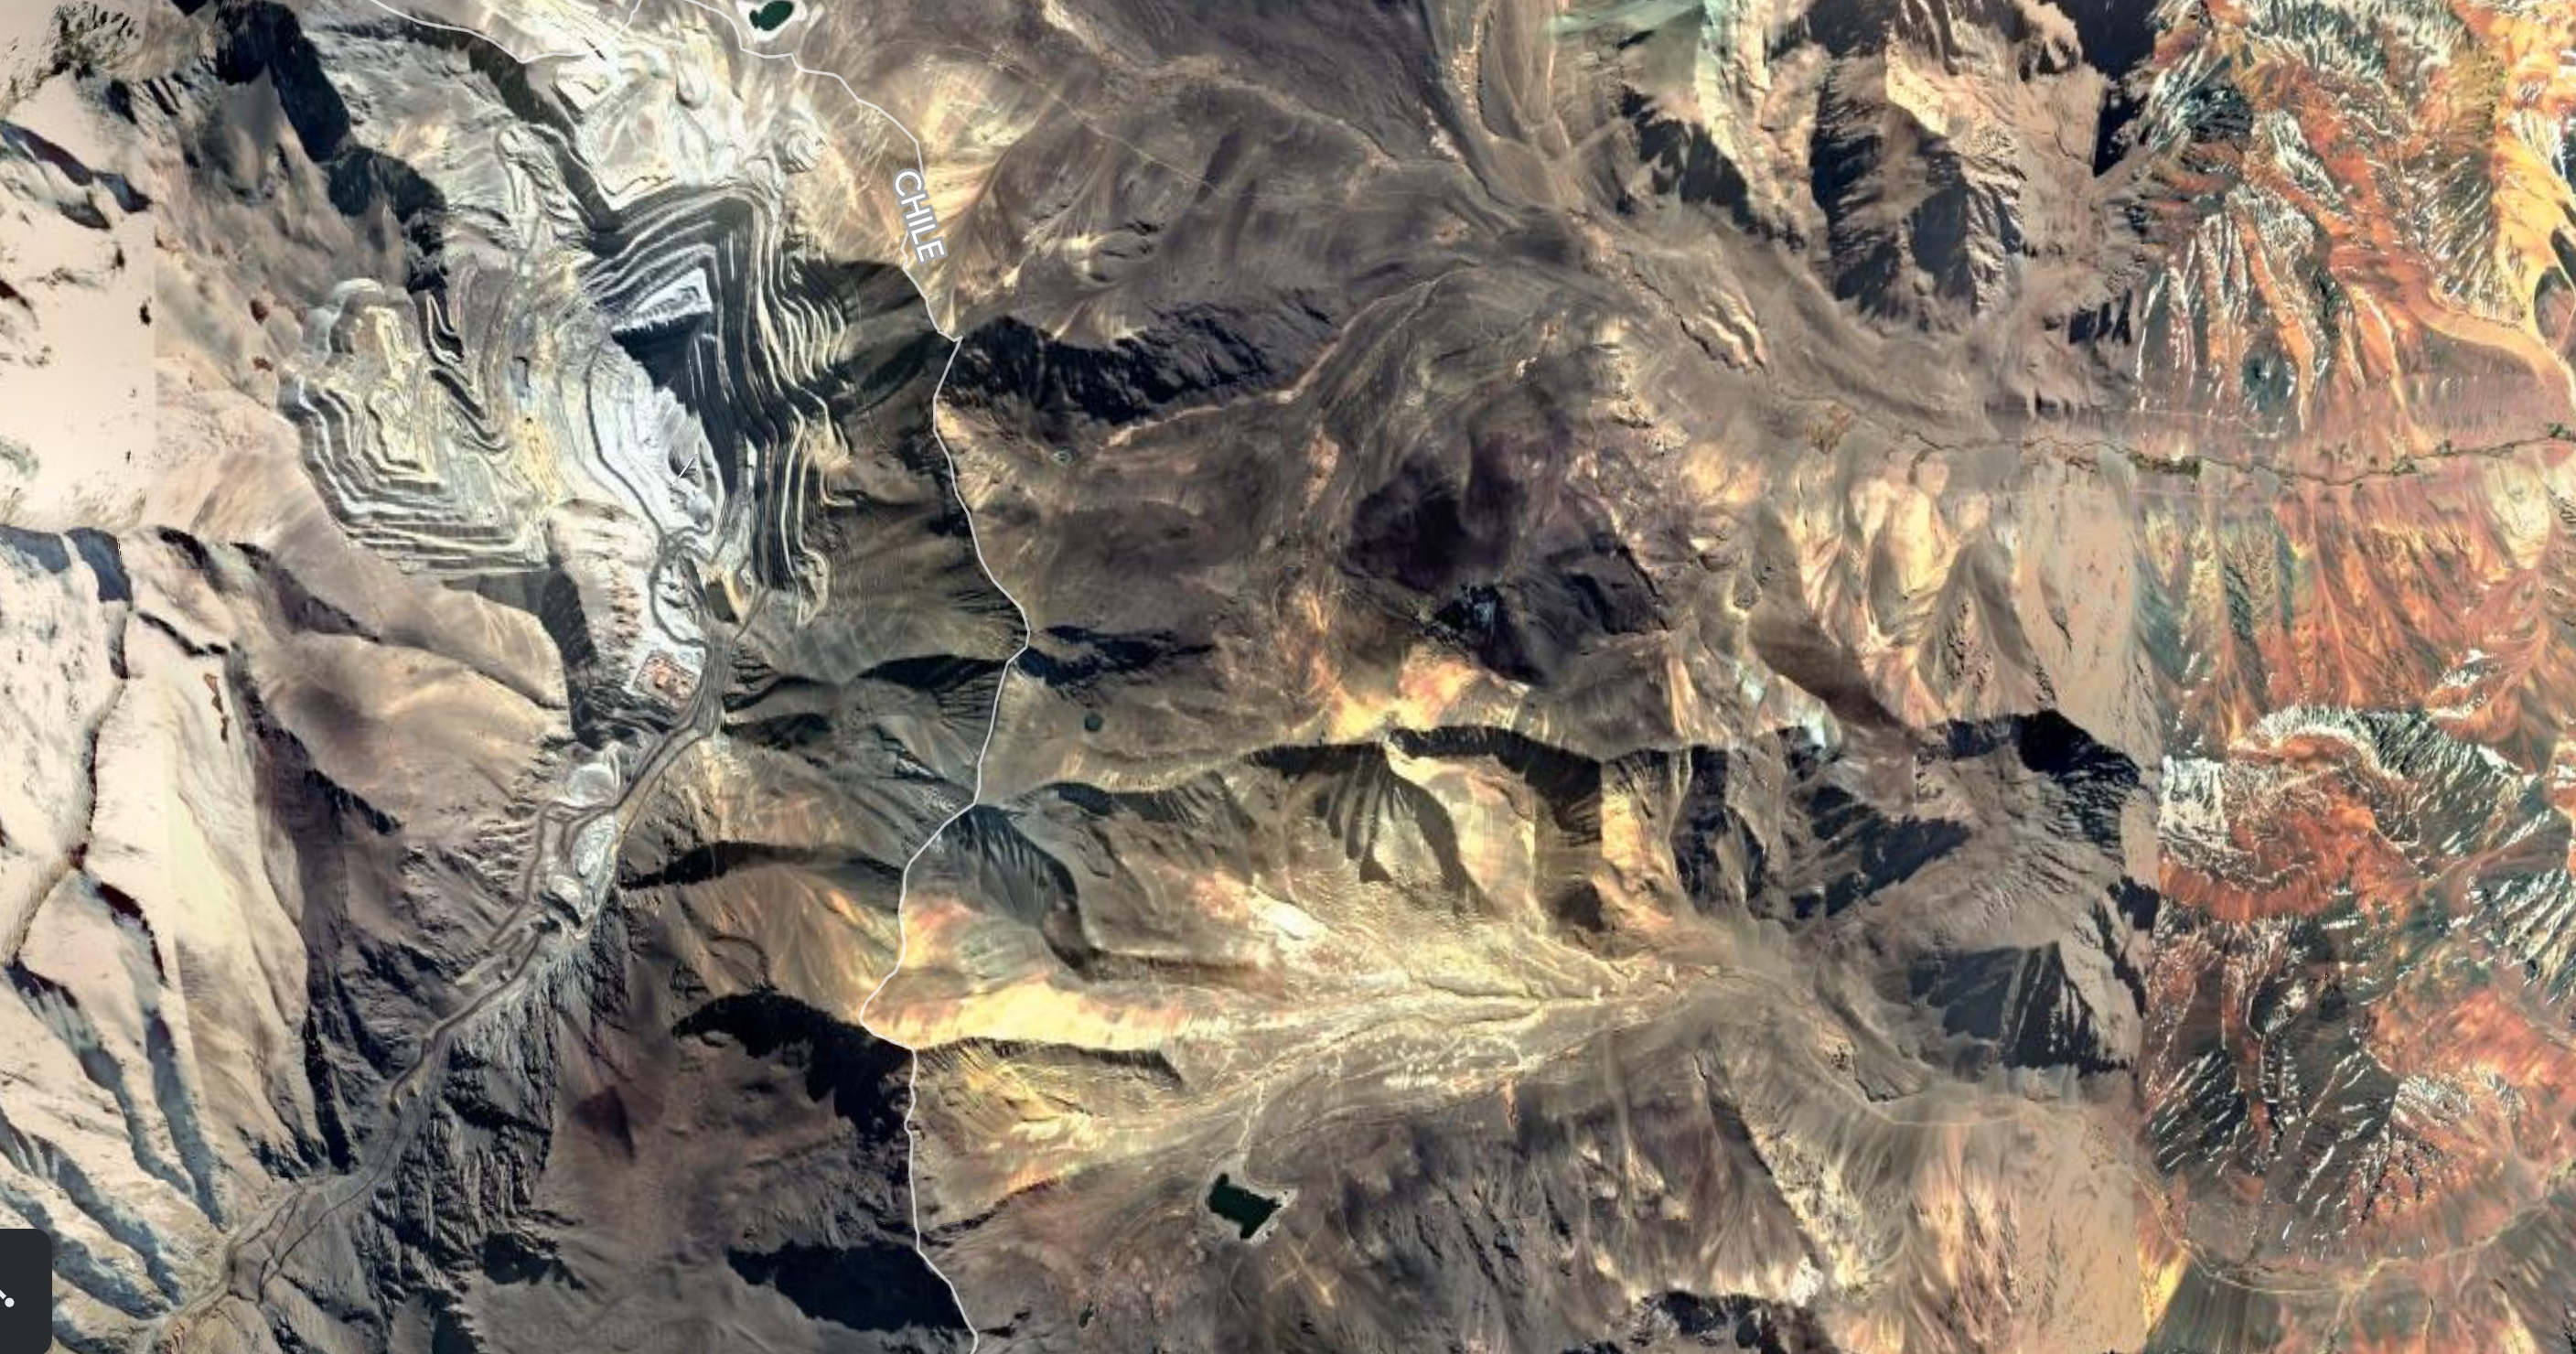
\includegraphics[scale=0.4]{Slides Principios de Economia/Figures/Mina.png}
\end{frame}

\begin{frame}
\frametitle{Cuál es la diferencia...}
\begin{itemize}
    \item Durante el 2022, el sector minero argentino alcanzó los US\$3.878 millones de exportaciones y empleó formalmente a 90 mil personas.
    \item En cambio, Chile que exportó US\$55.530 millones!!
    \item  Argentina es parte de la región más grande del continente americano con depósitos minerales metálicos. Pachón es una de las 10 mayores reservas de cobre del mundo. Se conoce desde 1960 pero todavía no se pudo poner en marcha.
    \item Los Pelambres funciona desde 1999 y en 2022 generó más de U\$S 3000 millones.
    \item  El año pasado, Chile exportó US\$43.891 millones y Perú US\$19.500 millones de cobre. 
\end{itemize}
\end{frame}



\begin{frame}
\centering
“Una de las conclusiones más interesantes del neoinstitucionalismo económico es que la política y la economía están inextricablemente relacionadas y que no podemos explicar el desempeño económico de una determinada sociedad sin considerar esta relación.” Douglas C. North
\end{frame}

\begin{frame}
\frametitle{Asignaciones e instituciones}
\begin{itemize}
    \item Una asignación es el resultado de una interacción económica, pero está determinada por distintos factores:\vspace{4mm}
    \begin{itemize}
        \item La tecnología y los recursos naturales determinan lo posible.\vspace{2mm}
        \item Pero las instituciones dificultan o facilitan el accionar de los agentes ...\vspace{4mm}
    \end{itemize}
    \item Generalmente, nos interesan dos aspectos sobre las instituciones:\vspace{4mm}
    \begin{itemize}
        \item Queremos describirlas: ¿Como afecta la asignaciones?\vspace{2mm} 
        \item Queremos evaluarlas: ¿Cuales son las mejores instituciones?
    \end{itemize}
\end{itemize} 
\end{frame}

%\begin{frame}
%\frametitle{Factores que determinan una asignación}
%\definecolor{Azul}{rgb}{0.1,0.1,0.6}
%\begin{itemize}
%    \item Instituciones
%    \item \textcolor{Azul}{Tecnología}
%    \item \textcolor{Azul}{Biología}
%    \item \textcolor{Azul}{Preferencias}
%\end{itemize} 
%\end{frame}

\begin{frame}
\frametitle{¿Qué es una institución?}
De acuerdo a North  son las reglas del juego en una sociedad Que reducen la incertidumbre
  
 
    \begin{itemize}
        \item Y como consecuencia reducen los costos de transacción, proporcionando una estructura a la vida cotidiana.\vspace{2mm}
        \item Definen y limitan el conjunto de opciones de los individuos.\vspace{2mm}
        \item Son creadas por seres humanos.\vspace{2mm}
        \end{itemize}
        \begin{itemize}
        \item Normas formales e informales.\vspace{2mm}
        \item Afectan la performance de la economía.\vspace{2mm}
        \end{itemize}
        \begin{itemize}
        \item Pueden inducir a aumentar o reducir la productividad.
        \end{itemize} 
 
\end{frame}

\begin{frame}
\frametitle{Formales o informales}
\centering
\includegraphics[scale=0.4]{Slides Principios de Economia/Figures/Mina2.png}
\end{frame}


\begin{frame}
\frametitle{¿Qué es una institución?}
\begin{itemize}
    \item Greif [2006] dio una definición más precisa:
    \\ \vspace{2mm}
    ``Una institución es un sistema de reglas, creencias, normas y organizaciones que juntas generan una regularidad en la conducta''\vspace{2mm}
    \\ \vspace{2mm}
    \item Una regularidad en el comportamiento social 
    \begin{itemize}
        \item Comportamiento en situaciones recurrentes...
        \item ... llevado a cabo por individuos que ocupan una posición social particular.\vspace{2mm}
    \end{itemize}
    \item Cada componente del sistema
    \begin{itemize}
        \item Es social al ser hecho por el hombre...
        \item ... y exógeno a cada individuo cuyo comportamiento influye
    \end{itemize}
\end{itemize} 
\end{frame}

\begin{frame}
\frametitle{Los componentes del sistema}
\begin{itemize}
    \item Las reglas, cuando son reconocidas socialmente, guían el comportamiento\vspace{2mm}
    \begin{itemize}
        \item Crean un conocimiento compartido.\vspace{2mm}
        \item Proveen información y coordinan el comportamiento.\vspace{2mm}
        \item Indican el comportamiento socialmente aceptable.\vspace{4mm}
    \end{itemize}
    \item Las creencias y normas motivan a seguir reglas\vspace{2mm}
    \begin{itemize}
        \item Normas y creencias internalizadas.\vspace{4mm}
    \end{itemize}
    \item Las organizaciones (formales o informales)\vspace{2mm}
    \begin{itemize}
        \item Producen y difunden reglas.\vspace{2mm}
        \item Perpetúan creencias y normas.\vspace{2mm}
        \item Influyen en el conjunto de creencias factibles.\vspace{2mm}
    \end{itemize}
\end{itemize}
\end{frame}

\begin{frame}
\frametitle{Discutamos ejemplos...}
\centering
\includegraphics[scale=0.45]{Slides Principios de Economia/Figures/Tema_04.1_examples.png}
\end{frame}

\begin{frame}
\frametitle{Importancia de las instituciones}
\begin{itemize}
    \item Al generar una regularidad en la conducta, las instituciones determinan qué tan grandes son los costos de transacción, y quien los paga\vspace{2mm}
    \begin{itemize}
        \item Esto afecta si los agentes actúan o no.\vspace{2mm}
        \item Buenas instituciones reducen los costos de transacción, lo que implica más transacciones económicas.\vspace{4mm}
    \end{itemize}
    \item ¿Importan para el crecimiento?
\end{itemize}
\end{frame}

\begin{frame}
\frametitle{El problema de simultaneidad}
\centering
\includegraphics[scale=0.35]{Slides Principios de Economia/Figures/Tema_04.1_examples2.png}
    \small Fuente: Acemoglu, Johnson & Robinson (2001)
\end{frame}

\begin{frame}
\frametitle{Asignaciones y justicia}
\begin{itemize}
    \item Una asignación puede ser considerada justa o injusta en sí \vspace{2mm}
    \begin{itemize}
        \item Un juicio substantivo de la justicia:\\ \vspace{2mm}
        - Necesitamos una métrica de "lo que nos parece bien o mal" \\
        - ¿Qué define que es justo?
    \end{itemize}
    \vspace{4mm}
    \item  Una asignación puede ser considerada justo o  injusta por la forma en que se llegó a ese resultado\vspace{2mm}
    \begin{itemize}
        \item Un juicio procedimental de la justicia \\
        - Necesitamos entender las reglas de juego y cómo se llegó al resultado \\
        - ¿Fueron los intercambios voluntarios?, ¿Fueron algunos individuos discriminados?, etc.
    \end{itemize}
    \item Quizás evaluamos diferente la riqueza de Elon Musk, la de Carlos Slim, o la de Lázaro Baez. 
\end{itemize}
\end{frame}

\begin{frame}
\frametitle{Economía y justicia}
\begin{itemize}
    \item Los valores que tiene la gente sobre lo que es justo y lo que no, varía entre individuos. ¿Podemos construir una teoría de la moral?\vspace{4mm}
    \item El filósofo americano John Rawls sugirió hacerlo en tres etapas:\vspace{2mm}
    \begin{itemize}
        \item El velo de la ignorancia: imaginarse detrás del velo de la ignorancia, es decir, imaginarse un tema sin saber que lugar ocuparemos en esa sociedad.\vspace{2mm}
        \item Elaboramos un juicio o evaluamos una institución desde atrás de ese velo.\vspace{4mm}
    \end{itemize}
    \item Por ejemplo: ¿los ricos deberían pagar más impuestos? ¿las personas con habilidades especiales deberían recibir una compensación del resto de la sociedad? 
\end{itemize}
\end{frame}

\begin{frame}
\frametitle{Economía y justicia}
\begin{itemize}
    \item La economía no hace juicios sobre lo que es justo o no pero sí puede ayudarnos a pensar una serie de cosas: \vspace{2mm}
    \begin{itemize}
        \item Cómo las instituciones (reglas del juego) afectan las asignaciones y la desigualdad.\vspace{2mm}
        \item  Cómo explotar todas las situaciones de win-win que no generan conflicto.\vspace{2mm}
        \item Qué tipo de políticas públicas son las mejores para lidiar con la injusticia
    \end{itemize}
\end{itemize}\end{frame}


\begin{frame}
\frametitle{Entendiendo el valor de las instituciones}
\begin{itemize}
    \item Arrancamos con una frontera de posibilidades de producción \vspace{4mm}
        \begin{itemize}
        \item La frontera factible nos indica lo que es tecnológicamente posible. \vspace{2mm}
        \item Pero ahora vamos a sumar una restricción que considera lo que es biológicamente posible.
        \begin{itemize} \vspace{4mm}
            \item ¿Qué significa esto? \\
            - Hay un mínimo de recursos que el individuo necesita para sobrevivir, aún si no produce nada...
            - ... y cuantas mas energías utiliza produciendo, más recursos va a necesitar
        \end{itemize}
    \end{itemize}
\end{itemize}
\end{frame}

\begin{frame}
\frametitle{La restricción biológica}
\centering
\begin{center}
\begin{figure}[H]
\renewcommand{\figurename}{Figure}
\begin{center}
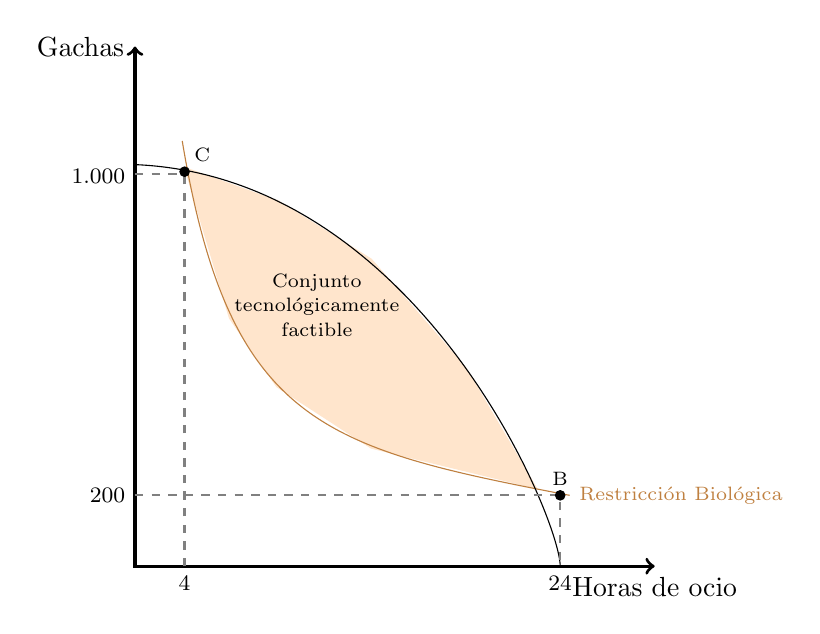
\begin{tikzpicture}[scale=0.6]
\draw[fill,orange!20] (1.05,8.45)--(2,5.25)--(3,3.8)--(5,2.5)--(8.5,1.65)--(7,4.2)--(5,6.5)--(3,7.75);
\draw[very thick,<->] (0,11) node[left]{Gachas}--(0,0)--(11,0) node[below]{Horas de ocio};
\draw[thin, brown] (1,9).. controls (2,3) and (4, 2.5) .. (9.2, 1.5) node[right]{\scriptsize Restricción Biológica};
\draw[thin] (0,8.5).. controls (6,8.25) and (9, 1) .. (9,0);
\draw[thick, dashed, gray] (0,1.5)--(9,1.5)--(9,0);
\draw[thick, dashed, gray] (1.05,0)--(1.05,8.25);
\draw[thick, dashed, gray] (0,8.3)--(1.05,8.3);
\node[below] at (1.05,0) {\footnotesize $4$};
\node[below] at (9,0) {\footnotesize 24};
\node[left] at (0,1.5) {\footnotesize $200$};
\node[left] at (0,8.25) {\footnotesize $1.000$};
\draw[fill] (9,1.5) circle [radius =0.1] node[above]{\scriptsize B};
\draw[fill] (1.05,8.35) circle [radius =0.1] node[above right]{\scriptsize C};
%\node[right] at (1,5) {\scriptsize Restricción Biológica};
\node[] at (3.85,6) {\scriptsize Conjunto};
\node[] at (3.85,5.5) {\scriptsize tecnológicamente};
\node[] at (3.85,5) {\scriptsize factible};
\end{tikzpicture}
\end{center}
\caption{Restricción biológica}
\label{fig:C11.6}
\end{figure}
\end{center}
\end{frame}


\begin{frame}
\frametitle{El objetivo es comparar distintas instituciones}
\begin{itemize}
        \item Comparamos escenarios donde:\vspace{2mm}
            \begin{itemize}
            \item Situaciones históricas\vspace{2mm}
            \begin{itemize}
            \item El régimen de esclavitud (Imperio Romano)\vspace{2mm}
            \item Campesinos libres (EEUU en el siglo XVIII)\vspace{2mm}
            \item Servidumbre con renta fija (Medioevo)\vspace{2mm}
            \item Servidumbre con renta variable (Medioevo)\vspace{2mm}
            \item La China comunista \vspace{2mm}
            \item Un país con sindicatos (Sudáfrica)\vspace{2mm}
            \end{itemize}
        \end{itemize}\vspace{4mm}
    \item ¿En qué forma queremos compararlas? Por ahora, en términos de eficiencia de Pareto
\end{itemize}
\end{frame}

\begin{frame}
\frametitle{¿Qué punto elige el dictador?}
\centering
\includegraphics[scale=0.4]{Slides Principios de Economia/Figures/Tema_04.7_modcap4_2.jpg}\end{frame}


\begin{frame}
\frametitle{¿Qué punto elige el dictador?}
\begin{center}
\begin{figure}[H]
\renewcommand{\figurename}{Figure}
\begin{center}
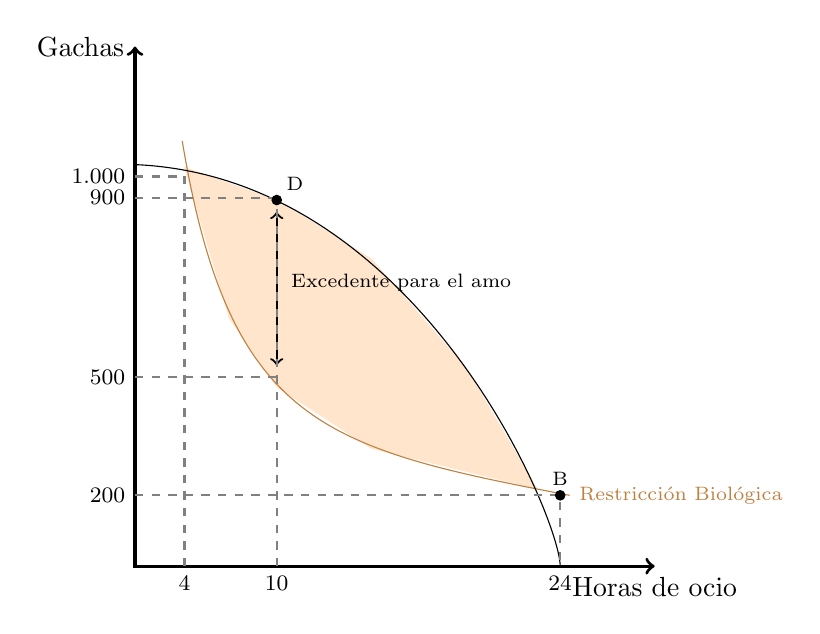
\begin{tikzpicture}[scale=0.6]
\draw[fill,orange!20] (1.05,8.45)--(2,5.25)--(3,3.8)--(5,2.5)--(8.5,1.65)--(7,4.2)--(5,6.5)--(3,7.75);
\draw[very thick,<->] (0,11) node[left]{Gachas}--(0,0)--(11,0) node[below]{Horas de ocio};
\draw[thin, brown] (1,9).. controls (2,3) and (4, 2.5) .. (9.2, 1.5) node[right]{\scriptsize Restricción Biológica};
\draw[thin] (0,8.5).. controls (6,8.25) and (9, 1) .. (9,0);
\draw[thick, dashed, gray] (0,1.5)--(9,1.5)--(9,0);
\draw[thick, dashed, gray] (1.05,0)--(1.05,8.25);
\draw[thick, dashed, gray] (0,8.25)--(1.05,8.25);
\node[below] at (1.05,0) {\footnotesize $4$};
\node[below] at (3,0) {\footnotesize $10$};
\node[below] at (9,0) {\footnotesize 24};
\node[left] at (0,1.5) {\footnotesize $200$};
\node[left] at (0,4) {\footnotesize $500$};
\node[left] at (0,8.25) {\footnotesize $1.000$};
\node[left] at (0,7.8) {\footnotesize $900$};
\draw[fill] (9,1.5) circle [radius =0.1] node[above]{\scriptsize B};
\draw[thick, <->] (3,4.25)--(3,7.5) ; 
\node[right] at (3.1,6) {\scriptsize Excedente para el amo};
\draw[thick, dashed, gray] (3,0)--(3,7.8);
\draw[thick, dashed, gray] (0,4)--(3,4);
\draw[thick, dashed, gray] (0,7.8)--(3,7.8);

\draw[fill] (3,7.75) circle [radius =0.1] node[above right]{\scriptsize D};
\end{tikzpicture}
\end{center}
\caption{Excedente}
\label{fig:C11.7}
\end{figure}
\end{center}
\end{frame}

\begin{frame}
\frametitle{El equilibrio de la esclavitud}
\centering
\centering
\includegraphics[scale=0.55]{Slides Principios de Economia/Figures/Instituciones1.jpg}
\end{frame}

%\begin{frame}
%\frametitle{El régimen de esclavitud}
%\centering
%\includegraphics[scale=0.4]{Slides Principios de Economia/Figures/Tema_04.8_modcap4_3.jpg}
%\end{frame}


\begin{frame}
\frametitle{Ahora el esclavo se libera!}
\begin{center}
\begin{figure}[H]
\renewcommand{\figurename}{Figure}
\begin{center}
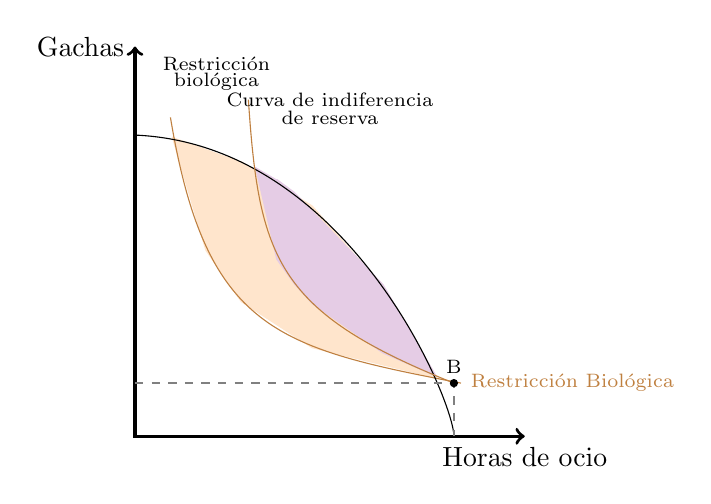
\begin{tikzpicture}[scale=0.45]
\draw[fill,orange!20] (1.05,8.45)--(2,5.25)--(3,3.8)--(5,2.5)--(8.5,1.65)--(7,4.2)--(5,6.5)--(3,7.75);
\draw[fill,violet!20] (3.4,7.6)--(4,5)--(4.5,4.3)--(5,3.75)--(7,2.35)--(8.5,1.7)--(7,4.28)--(4.5,6.88)--(4,7.25);
\draw[very thick,<->] (0,11) node[left]{Gachas}--(0,0)--(11,0) node[below]{Horas de ocio};
\draw[thin, brown] (1,9).. controls (2,3) and (4, 2.5) .. (9.2, 1.5) node[right]{\scriptsize Restricción Biológica};
\draw[thin] (0,8.5).. controls (6,8.25) and (9, 1) .. (9,0);

\draw[thin, brown] (3.2,9.5).. controls (3.5,5) and (4, 3.5) .. (9, 1.5);
\draw[thick, dashed, gray] (0,1.5)--(9,1.5)--(9,0);
\draw[fill] (9,1.5) circle [radius =0.1] node[above]{\scriptsize B};
\node[] at (5.5,9.5) {\scriptsize Curva de indiferencia};
\node[] at (5.5,9) {\scriptsize  de reserva};
\node[] at (2.3,10.5) {\scriptsize Restricción};
\node[] at (2.3,10) {\scriptsize  biológica};
\end{tikzpicture}
\end{center}
\end{figure}
\end{center}
\begin{itemize}
    \item Ahora el campesino toma en cuenta la desutilidad del trabajo. Puede decidir no hacerlo.
    \item Toma en cuenta el costo de oportunidad. El trabajador tiene otros ingresos u opciones que le garantizan la supervivencia.
\end{itemize}
\end{frame}


\begin{frame}
\frametitle{Ahora tengo en cuenta las preferencias del trabajador}
\begin{itemize}
        \item ¿Cómo lucen las preferencias? \vspace{2mm}
        \begin{itemize}
            \item Vamos a hacer un supuesto sobre la forma de las curvas de indiferencia para simplificar toda la interpretación \\ \vspace{2mm}
            - Tener más o menos producto no va a afectar la valuación del ocio, es decir, valoramos el ocio siempre igual, independientemente del nivel de producto (es decir, TMS constante para un nivel de ocio)
        \end{itemize}
\end{itemize}
\end{frame}

\begin{frame}
\frametitle{Preferencias cuasi-lineales}
\centering
\includegraphics[scale=0.3]{Slides Principios de Economia/Figures/Tema_04.5_prefcuasilin.jpg}
\end{frame}


\begin{frame}
\frametitle{La decisión del campesino libre}
\begin{center}
\begin{figure}[H]
\renewcommand{\figurename}{Figure}
\begin{center}
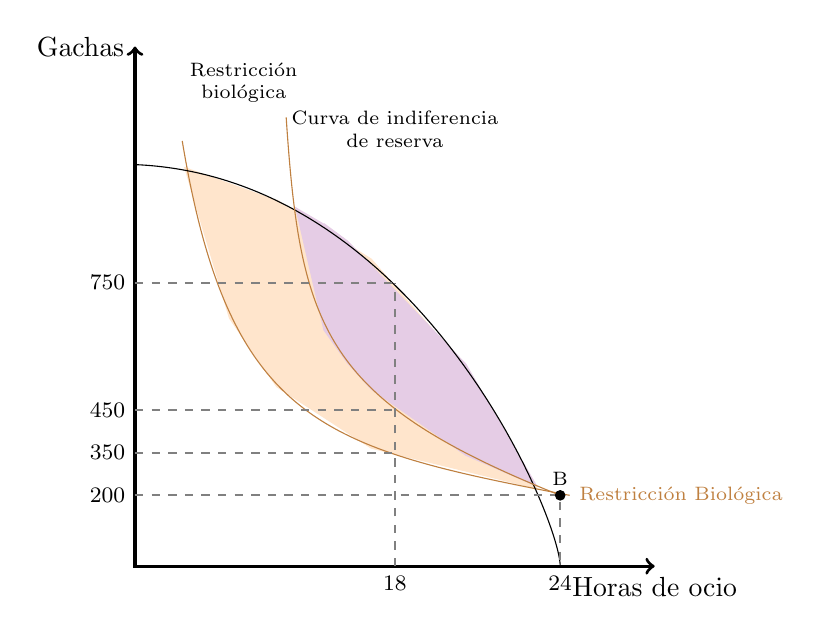
\begin{tikzpicture}[scale=0.6]
\draw[fill,orange!20] (1.05,8.45)--(2,5.25)--(3,3.8)--(5,2.5)--(8.5,1.65)--(7,4.2)--(5,6.5)--(3,7.75);
\draw[fill,violet!20] (3.4,7.6)--(4,5)--(4.5,4.3)--(5,3.75)--(7,2.35)--(8.5,1.7)--(7,4.28)--(4.5,6.88)--(4,7.25);
\draw[very thick,<->] (0,11) node[left]{Gachas}--(0,0)--(11,0) node[below]{Horas de ocio};
\draw[thin, brown] (1,9).. controls (2,3) and (4, 2.5) .. (9.2, 1.5) node[right]{\scriptsize Restricción Biológica};
\draw[thin] (0,8.5).. controls (6,8.25) and (9, 1) .. (9,0);

\draw[thin, brown] (3.2,9.5).. controls (3.5,5) and (4, 3.5) .. (9, 1.5);
\draw[thick, dashed, gray] (0,1.5)--(9,1.5)--(9,0);
%\draw[thick, dashed, gray] (1.05,0)--(1.05,8.25);
%\draw[thick, dashed, gray] (0,8.25)--(1.05,8.25);
%\node[below] at (1.05,0) {\footnotesize $4$};
\node[below] at (5.5,0) {\footnotesize $18$};
\node[below] at (9,0) {\footnotesize 24};
\node[left] at (0,1.5) {\footnotesize $200$};
\node[left] at (0,2.4) {\footnotesize $350$};
\node[left] at (0,3.3) {\footnotesize $450$};
\node[left] at (0,6) {\footnotesize $750$};
%\node[left] at (0,8.25) {\footnotesize $1.000$};
%\node[left] at (0,7.8) {\footnotesize $900$};
\draw[fill] (9,1.5) circle [radius =0.1] node[above]{\scriptsize B};
%\draw[thick, <->] (3,4.25)--(3,7.5);
\draw[thick, dashed, gray] (5.5,0)--(5.5,6);
\draw[thick, dashed, gray] (0,6)--(5.5,6);
\draw[thick, dashed, gray] (0,3.3)--(5.5,3.3);
\draw[thick, dashed, gray] (0,2.4)--(5.5,2.4);
%\draw[thick, dashed, gray] (0,7.8)--(3,7.8);
\node[] at (5.5,9.5) {\scriptsize Curva de indiferencia};
\node[] at (5.5,9) {\scriptsize  de reserva};
\node[] at (2.3,10.5) {\scriptsize Restricción};
\node[] at (2.3,10) {\scriptsize  biológica};
%\node[] at (4.9,5.45) {\tiny Conjunto};
%\node[] at (5.2,5) {\tiny económicamente};
%\node[] at (5.5,4.55) {\tiny posible};

\end{tikzpicture}
\end{center}
\end{figure}
\end{center}
\end{frame}

\begin{frame}{Las diferencias entre la esclavitud y la libertad}
\centering
\includegraphics[scale=0.55]{Slides Principios de Economia/Figures/Instituciones2.jpg}
\end{frame}


\begin{frame}{Las diferencias entre la esclavitud y la libertad}
\begin{itemize}
    \item Como la utilidad es cuasilineal se maximiza la utilidad maximizando la diferencia entre la producción y la curva de indiferencia de reserva
     \item El punto máximo es cuando se iguala la pendiente de la curva de transformación con la de la curva de indiferencia de reserva. 
    \item El dueño de la tierra trabaja menos que en el régimen de esclavitud.\vspace{4mm}
    \item Pero eso es óptimo: porque el régimen de esclavitud no tomaba en cuenta su desutilidad! \vspace{4mm}
    \item  El cambio de instituciones cambió la asignación (y la distribución).
\end{itemize}
\end{frame}


\begin{frame}
\frametitle{Servidumbre medieval: servidumbre fija }
\begin{itemize}
    \item Estamos en la edad media donde un señor feudal es dueño de la tierra. 
\item Se le permite a un campesino trabajar la tierra pero a cambio de una "servidumbre". 
    \item  En este caso asumimos que el pago es un monto fijo de producción 
    \item Reduce lo que se lleva el campesino desplazando su retorno hacia abajo.
    \item La producción no se modifica pero sí su distribución (ahora el campesino tiene que pasarle parte al señor feudal). 
\end{itemize}
\end{frame}

\begin{frame}
\frametitle{Servidumbre medieval: servidumbre fija }
\centering
\includegraphics[scale=0.55]{Slides Principios de Economia/Figures/Instituciones3.jpg}
\end{frame}

\begin{frame}
\frametitle{Servidumbre medieval: un porcentaje de la producción }
\begin{itemize}
    \item Ahora asumimos que el pago es un porcentaje de la producción 
    \item Reduce lo que se lleva el campesino desplazando su retorno hacia abajo pero no de manera paralela sino que lo que se reduce crece con la producción
    \item La producción ahora cae respecto al caso anterior
     \item Hay una distorsión en la producción pero el riesgo está mejor distribuido entre productor y sr feuda. 
\end{itemize}
\end{frame}

\begin{frame}
\frametitle{Servidumbre medieval: un porcentaje de la producción}
\centering
\includegraphics[scale=0.6]{Slides Principios de Economia/gachas.png}
\end{frame}



\begin{frame}
\frametitle{Diversificando riesgo en la Edad Media}
\centering
\includegraphics[scale=0.4]{Slides Principios de Economia/PastedGraphic-1.pdf}

\begin{itemize}
    \item Una manera de acotar el riesgo era partiendo las parcelas y distribuyéndolas en un área geográfica más amplia. 
\end{itemize}
\end{frame}

\begin{frame}
\frametitle{La China de Mao}
\begin{center}
\begin{figure}[H]
\renewcommand{\figurename}{Figure}
\begin{center}
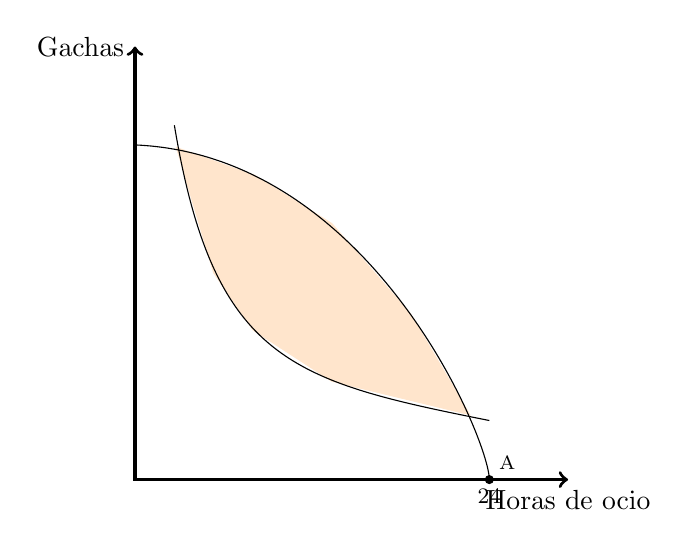
\begin{tikzpicture}[scale=0.5]
\draw[fill,orange!20] (1.05,8.45)--(2,5.25)--(3,3.8)--(5,2.5)--(8.5,1.65)--(7,4.2)--(5,6.5)--(3,7.75);
\draw[very thick,<->] (0,11) node[left]{Gachas}--(0,0)--(11,0) node[below]{Horas de ocio};
\draw[thin] (1,9).. controls (2,3) and (4, 2.5) .. (9, 1.5);
\draw[thin] (0,8.5).. controls (6,8.25) and (9, 1) .. (9,0);
%\draw[fill] (8.5,1.6) circle [radius =0.1] node[left]{$A$};
\draw[fill] (9,0) circle [radius =0.1];
%\draw[thick, <->] (4.5,0.15)--(4.5,4.35);
%\draw[thick, <->] (4.5,6.75)--(4.5,4.65);
\node[above right] at (9,0) {\scriptsize A};
%\node[] at (3.55,5.5) {\scriptsize dictador};
%\node[] at (3.5,2) {\scriptsize Para el};
%\node[] at (3.4,1.5) {\scriptsize productor};
\node[below] at (9,0) {\footnotesize 24};
%\node[below] at (8.5,0) {\footnotesize 23};
%\node[left] at (0,1.6) {\footnotesize 120 gr};
%\draw[thin, dashed, gray] (0,1.6)--(8.5,1.6);
%\draw[thin, dashed, gray] (8.5,0)--(8.5,1.6);
\end{tikzpicture}
\end{center}
\label{fig:C11.15}
\end{figure}
\end{center}
\end{frame}

\begin{frame}
\frametitle{La China de Mao }
\begin{itemize}
    \item Cuando Mao llega al poder decide la colectivización de las granjas
    \item Lo que recibe cada productor es independiente de lo que produce. 
    
    \item El productor maximiza su utilidad minimizando su trabajo 
     \item La producción baja a cero.  
     \item 40 millones de personas murieron de hambre
     \item ¡Vaya si las instituciones importan! 
\end{itemize}

\end{frame}

\begin{frame}
\frametitle{¿Qué pasa si hay un salario mínimo o un bono obligatorio?}
\centering
\includegraphics[scale=0.33]{Slides Principios de Economia/Figures/InstitucionesBono.png}
\end{frame}

\begin{frame}
\frametitle{¿Qué pasa si hay un salario mínimo o un bono obligatorio?}
\centering
\includegraphics[scale=0.8]{Slides Principios de Economia/Figures/Salariominimo.png}
\end{frame}

\begin{frame}
\frametitle{El gobierno sindical de Sudáfrica}
\begin{itemize}
    \item La remuneración de los trabajadores la define un "sindicato". 
    \item  Asumimos esa remuneración es mayor a la que ocurriría naturalmente
    \item Definido el salario el dueño de la tierra define cuanto producir
    \item  La producción cae, pero la parte de la torta que se lleva el trabajador puede subir. 
\end{itemize}
\end{frame}

\end{document}
